\chapter{Technické předpoklady}

\section{Resource Description Framework}
Resource Description Framework, zkráceně RDF, je rodina specifikací\footnote{\citet{Raimond:14:RP}} (tedy sada pravidel), která se používá na popis informací na internetu. RDF popisuje data jako graf, konkrétně vrcholy grafu jsou entity, jež ztvárňují nějaké věci (fyzické předměty, díla, myšlenky) a hrany tyto entity propojují a dávají jim vztahy.

Základem je takzvaný \textbf{statement} (česky tvrzení). Tvrzení je vyjádřeno formou trojice v tomto pořadí ze subjektu, predikátu a objektu, přičemž subjekt a objekt jsou vrcholy (anglicky \textbf{nodes}) a predikát je orientovanou hranou jdoucí od subjektu k objektu.

Vrcholem v RDF může být IRI, literál, nebo prázdný vrchol.

\medskip

Jako vrchol IRI (Internationalized Resource Identifier) se rozumí vrchol, jež přiřazuje entitě nějaký identifikátor ve tvaru IRI. Tímto jsme schopni v rámci WWW identifikovat různé entity a pracovat s nimi napříč různými zdroji. Ku příkladu Karel Čapek, zmíněný v úvodu, je v rámci Wikidat jednoznačně identifikován jako \url{https://www.wikidata.org/wiki/Q155855}. IRI kromě identifikátoru nenese žádné další informace včetně jména, reprezentuje tedy nějakou entitu, která musí být popsaná tvrzeními, aby dostala význam.

\medskip

Literálem je pak vrchol nesoucí nějakou hodnotu. Může se jednat o číslo popisující věk osoby, její jméno atp. V rámci RDF kromě hodnoty má literál i svůj typ, jež je opět vyjádřen pomocí IRI. Uveďme kupříkladu \url{http://www.w3.org/2001/XMLSchema#integer} jež vyjadřuje obecně celé číslo. Speciálním typem je \url{http://www.w3.org/1999/02/22-rdf-syntax-ns#langString}, který vyžaduje ještě takzvaný \textbf{laguage tag} a popisuje text v nějakém konkrétním jazyce.

\medskip

Literály nám tedy dávají možnost popsat IRI vrcholy (entity) pomocí různých vlastností, které podporují právě i multijazyčnost. S pomocí takovýchto grafů pak dokážeme popsat celou řadu věcí z reálného světa.

Nakonec, hrana je opět popsána pomocí IRI, jež reprezentuje typ vztahu.

\subsection{Turtle jazyk}
RDF graf může být popsán pomocí Turtle jazyka\footnote{\citet{Prud'hommeaux:14:RT}}. Ten je využit při zápisu konfigurací, jež jsou popsány dále v tomto dokumentu.

Trojice (tvrzení) se zapisují jako tři slova oddělená mezerami a zakončená tečkou. Chceme-li zapsat IRI, musíme jej dát do špičatých závorek \texttt{<>}. Na začátku dokumentu lze definovat prefixy, které pak umožňují zkrátit zapisované IRI do namespace a zbylé části jako \texttt{namespace:zbytek}.

Pokud se nám u trojic opakuje subjekt a predikát, můžeme jednotlivé objekty oddělovat čárkou (\texttt{,}). Obdobně, pokud se nám opakuje jen subjekt, můžeme dvojice predikát-objekt oddělovat středníkem (\texttt{;}).

\newpage

Uveďme několik příkladů RDF grafu.

\begin{prikl}
Tvrzení \uv{Karel Čapek se narodil 9. ledna 1890} vyjádřené v rámci Wikidat.
\begin{code}
@prefix wd: <https://www.wikidata.org/wiki/> .
@prefix wdt: <https://www.wikidata.org/wiki/Property:> .
@prefix xsd: <http://www.w3.org/2001/XMLSchema#> .

wd:Q155855 wdt:P569 "1890-01-09"^^xsd:dateTime .
\end{code}

Kód popisuje jedno tvrzení, kdy se Karlu Čapkovi \\ \url{https://www.wikidata.org/wiki/Q155855} přiřadí přes property datum narození \url{https://www.wikidata.org/wiki/Property:P569} literál s jeho datem narození, jež má typ \url{http://www.w3.org/2001/XMLSchema#dateTime}.
\end{prikl}

Jak lze vidět z příkladu, tvrzení nemusí odkazovat jen na svůj dataset, ale i mimo něj. To nám dovoluje stavět již na existujících datasetech a jednoduše se na ně odkazovat přes IRI. Můžeme tak mít vlastní knihovní databázi, jež ke knize přiřadí autora z datasetu Wikidat. Tímto jsme propojili dva datasety, což nám umožní nad nimi provádět dotazy. Příkladem takového dotazu by mohlo být \uv{Chci seznam knih v naší knihovně, jež byly napsány českými autory.} Takový dotaz pak současně prohledá dva různé datasety a vrátí očekávané výsledky.

Uveďme ještě příklad tvrzení, jež se odkazuje na další entity.
\begin{prikl}
Tvrzení \uv{Děti Antonína Čapka jsou Karel, Josef a Helena} vyjádřené v rámci Wikidat.
\begin{code}
@prefix wd: <https://www.wikidata.org/wiki/> .
@prefix wdt: <https://www.wikidata.org/wiki/Property:> .

wd:Q6657059 wdt:P40 wd:Q155855 ,
                    wd:Q454568 ,
                    wd:Q4532606 .
\end{code}
\end{prikl}

\begin{figure}[h]
    \centering
    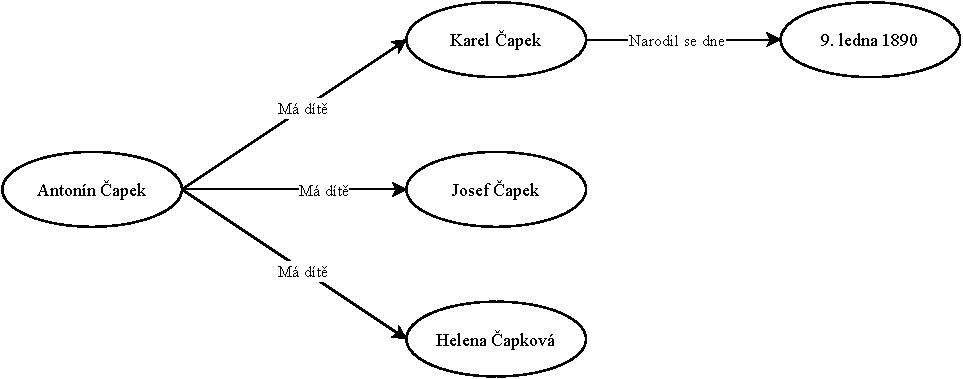
\includegraphics[width=\textwidth]{media/rdf.pdf}
    \caption{Příklad grafu, který získáme z předešlých dvou ukázek.}
\end{figure}

Pro úplnost zmiňme ještě následující graf popisující vztahy mezi lidmi, které jsou vyjádřeny ontologií FOAF (friend of a friend). Pokud by všechny zdroje popisující lidi využívaly tuto ontologii, měli bychom jednotné rozhraní, jak přistupovat k lidským vztahům.

Ontologie je slovník obsahující formalizovaný seznam pojmů na definici kategorií a vztahů z určitého oboru.

\begin{code}
@prefix foaf: <http://xmlns.com/foaf/0.1/> .
@prefix example: <http://example.org/> .

<http://example.org/Jan-Novák> foaf:name "Jan Novák" .
<http://example.org/Ondřej-Novák> foaf:name "Ondřej Novák" .

example:Pavel-Novotný foaf:name "Pavel Novotný" ;
                      foaf:knows example:Jan-Novák ,
                                 example:Ondřej-Novák .
\end{code}

\subsection{SPARQL jazyk}\label{SPARQL}
Jazyk SPARQL\footnote{\citet{Seaborne:13:SQL}} slouží k definici dotazů nad RDF daty a jejich manipulaci.

SPARQL má 4 typy dotazů:
\begin{itemize}
    \item \texttt{SELECT} dotaz vrací data z databáze ve formě tabulky obdobně jako u tabulkových databází. Můžeme tak například k jedné entitě vrátit hned několik vlastností jako různé sloupce tabulky.
    \item \texttt{CONSTRUCT} dotaz vrací data ve formě RDF grafu. Tento dotaz tedy použijeme, pokud chceme s výsledkem dále pracovat jako s grafem.
    \item \texttt{ASK} dotaz vrací pravdivostní hodnotu ano/ne podle toho, zda dotaz uspěl. Může být využit například ke zjištění, zda se konkrétní data již v databázi nacházejí.
    \item \texttt{DESCRIBE} dotaz obdobně jako \texttt{CONSTRUCT} vrací RDF graf s tím rozdílem, že zde určuje databáze, jaká data na dotaz dostaneme. Tento dotaz použijeme, pokud neznáme strukturu grafu a chceme získat \uv{nějaké} informace o vrcholu.
\end{itemize}

\newpage

\begin{prikl}
Dotaz, jež nám vrátí seznam děl Karla Čapka a jejich data vydání z Wikidat.
\begin{code}
PREFIX wd: <https://www.wikidata.org/wiki/>
PREFIX wdt: <https://www.wikidata.org/wiki/Property:>

SELECT ?title ?publication_date
WHERE
{
    wd:Q155855 wdt:P800 ?work .
    ?work wdt:P1476 ?title ;
          wdt:P577 ?publication_date .
}
\end{code}
Jedná se o \texttt{SELECT} dotaz, tedy jako výsledek dostaneme tabulku, jež má sloupce \texttt{title} a \texttt{publication_date}.

Dotaz se nejprve zeptá na všechny vrcholy, které dostaneme přes vlastnost \texttt{wdt:P800}, kterou Wikidata definují jako \uv{dílo - významné vědecké, umělecké či jiné dílo}. Tyto vrcholy jsou pak reprezentovány proměnnou \texttt{?work}. Na dalších dvou řádcích se pak dotazujeme, jaký titulek (\texttt{wdt:P1476}) má \texttt{?work} a uložíme ho do \texttt{?title}, který je i prvním sloupcem výstupu. Dále se pak obdobně ptáme na datum publikace, které je také součástí výsledku.
\end{prikl}

\begin{prikl}
Dotaz, zda vrchol identifikován jako \uv{Q7377} je taxon, nebo klad (dle Wikidat definovaný jako \uv{systematická jednotka v biologii zahrnující společného předka a všechny z něho vzešlé potomky}).
\begin{code}
ASK {
  wd:Q7377 wdt:P31 ?type .
  FILTER(?type IN (wd:Q16521, wd:Q713623))
}
\end{code}
Protože jako odpověď očekáváme ano/ne, jedná se o \texttt{ASK} dotaz. Obdobně jako v minulém příkladu ve \texttt{WHERE} části popisujeme podmínky, které pak určí, zda existuje nějaká trojice a tedy zda dotaz vrátí kladný výsledek. Všimněme si funkce \texttt{FILTER}, která dovoluje typu mít jen jednu ze dvou hodnot.
\end{prikl}

\begin{prikl}
Dotaz, který vrací graf dětí Antonína Čapka (\texttt{Q6657059}) v ontologii \url{http://purl.org/vocab/relationship/}.
\begin{code}
PREFIX relationship: <http://purl.org/vocab/relationship/>
CONSTRUCT {
    ?child relationship:childOf wd:Q6657059 .
} WHERE {
    wd:Q6657059 wdt:P40 ?child .
}
\end{code}
Nejprve specifikujeme, jak chceme, aby výsledný graf vypadal. Poté ve \texttt{WHERE} části určíme podmínky a tím i proměnné použité v první části dotazu.
\end{prikl}